% ============================================================
\chapter{Proposed Framework}
\label{ch:framework}
\label{ch:models}
% ============================================================

This chapter describes the demand prediction models and ensemble strategies that constitute the EnsembleNet framework. Individual model configurations are detailed first, followed by the two-stage LR-LSTM hybrid architecture and the six ensemble strategies.

\section{Individual Models}

Eight individual models are trained using \texttt{scikit-learn}~\parencite{scikit-learn}, as summarised in \autoref{tab:individual_models}. Each model is trained on the same chronologically split feature matrix, ensuring that performance differences reflect modelling capacity rather than differences in data access. All preprocessing steps, including standardisation for linear models and the construction of lag and cyclic temporal features, are applied identically across the model family to isolate the effect of the learning algorithm.

The eight models span four inductive-bias families, each included to establish a distinct performance baseline and to supply diverse base learners for the ensemble strategies evaluated in \autoref{sec:ensembles}.

\paragraph{Linear models (LR, Ridge, Lasso).} Ordinary least squares and its regularised variants serve as interpretable baselines that test how much predictive variance is captured by the engineered feature set alone. Linear models assume additive relationships between lag features, cyclical time encodings, spatial centroids, and weather indicators; if they achieve high $R^2$, much of the demand signal is deterministic rather than requiring non-linear function approximation. Ridge ($\ell_2$), and Lasso ($\ell_1$) regularisation~\parencite{hoerl1970ridge,tibshirani1996lasso} test whether multicollinearity among lag features or spatial coordinates degrades the OLS solution; near-identical performance across the three linear variants would indicate that regularisation offers negligible benefit once features are well engineered.

\paragraph{Tree-based models (Decision Tree, Random Forest).} An unpruned decision tree provides a non-linear baseline without ensemble averaging, revealing whether a single recursive partition can capture demand interactions. Random Forest~\parencite{breiman2001rf} extends this with 200-tree bagging to reduce variance; its inclusion tests whether bootstrap aggregation of shallow trees improves upon a single deep tree. Tree-based methods are expected to excel at modelling threshold effects (such as the sharp demand increase at morning rush hour), but may overfit sparse cluster-bin combinations where few training observations exist.

\paragraph{Boosting models (XGBoost, Gradient Boosting).} XGBoost~\parencite{chen2016xgboost} and scikit-learn Gradient Boosting~\parencite{friedman2001gbm} represent the current state of the art for tabular prediction tasks. Both build sequential ensembles of weak learners that correct residual errors from prior iterations; XGBoost adds $\ell_1$ and $\ell_2$ regularisation, column subsampling, and efficient sparse-matrix support. Their inclusion is motivated by the strong individual performance reported by~\parencite{liu2021epidemic} on NYC taxi data and by the expectation that gradient-boosted trees will capture non-linear interactions among lag, temporal, and spatial features that linear models cannot represent.

\paragraph{Hybrid model (LR-LSTM).} The LR-LSTM Hybrid~\parencite{kim2020hybrid,hochreiter1997long} decomposes demand into a linear trend and a non-linear residual modelled by an LSTM. It is included both as a standalone competitor and as the architectural template for the XGBoost-LSTM variant. The hybrid tests whether explicit residual decomposition (separating predictable linear structure from sequential dynamics) adds value beyond end-to-end gradient boosting, addressing RQ2 directly.

Including models from all four families ensures that the ensemble base-learner pool spans complementary inductive biases: linear models capture low-demand off-peak structure, tree-based models capture rush-hour threshold effects, and the hybrid captures sequential residual dynamics. This diversity is a prerequisite for effective ensemble combination~\parencite{wolpert1992stacking}, because meta-learners can only improve upon individual models when base-learner errors are partially independent.

\begin{table}[t]
\centering
\caption{Individual forecasting models and their configurations.\label{tab:individual_models}}
\begin{tabularx}{\textwidth}{>{\raggedright\arraybackslash}p{2.2cm} >{\raggedright\arraybackslash}X}
\toprule
\textbf{Model} & \textbf{Description} \\
\midrule
Linear Regression & Ordinary least squares baseline \\
Ridge~\parencite{hoerl1970ridge} & Linear regression with $\ell_2$ regularisation, $\alpha=1.0$ \\
Lasso~\parencite{tibshirani1996lasso} & Linear regression with $\ell_1$ regularisation, $\alpha=0.01$ \\
Decision Tree & Unpruned tree; baseline for tree-based methods \\
Random Forest~\parencite{breiman2001rf} & 200-tree bagging ensemble \\
XGBoost~\parencite{chen2016xgboost} & Gradient-boosted trees with $\ell_1/\ell_2$ regularisation \\
Gradient Boosting~\parencite{friedman2001gbm} & Sequential residual boosting via scikit-learn GBM \\
LR-LSTM Hybrid~\parencite{hochreiter1997long} & Two-stage residual architecture; see \autoref{sec:lrlstm} \\
\bottomrule
\end{tabularx}
\end{table}

\autoref{tab:hyperparams} documents the full hyperparameter specification for all 14 models, covering both individual estimators and ensemble strategies. For tree-based models, the number of estimators is set to 200 to balance bias and variance without incurring prohibitive training time. For the LSTM component of the LR-LSTM Hybrid, a lookback window of 10 time steps is used alongside an architecture of two stacked LSTM layers with interleaved dropout, trained with Adam at a learning rate of $10^{-3}$ and early stopping with a patience of 5 epochs. Ensemble meta-learners are uniformly instantiated as Ridge regression with $\alpha{=}1.0$, providing a regularised but interpretable second-stage estimator that is unlikely to overfit the meta-feature space.

\begin{table}[t]
\centering
\caption{Hyperparameter specifications for all 14 models (Individual and Ensemble). RF = Random Forest, GBM = Gradient Boosting, XGB = XGBoost, seq\_len = LSTM input sequence length.\label{tab:hyperparams}}
\footnotesize
\setlength{\tabcolsep}{4pt}
\begin{tabularx}{\textwidth}{@{}
 >{\raggedright\arraybackslash}p{2.4cm}
 >{\raggedright\arraybackslash}p{1.5cm}
 >{\raggedright\arraybackslash}X
 >{\raggedright\arraybackslash}p{2.2cm} @{}}
\toprule
\textbf{Model} & \textbf{Type} & \textbf{Key Hyperparameters} & \textbf{Notes} \\
\midrule
Linear Regression & Individual & \texttt{fit\_intercept=True} (sklearn defaults) & OLS baseline \\
Ridge & Individual & \texttt{alpha=1.0, max\_iter=1000} & $\ell_2$ regularisation \\
Lasso & Individual & \texttt{alpha=0.01, max\_iter=1000} & $\ell_1$ regularisation \\
Decision Tree & Individual & \texttt{criterion='squared\_error', max\_depth=None} & Unpruned \\
Random Forest & Individual & \texttt{n\_estimators=200, n\_jobs=-1, random\_state=42} & Bagging, bootstrapped \\
XGBoost & Individual & \texttt{n\_estimators=200, lr=0.1, max\_depth=6, subsample=0.8, colsample=0.8, reg\_alpha=0.1, reg\_lambda=1.0} & L1+L2 regularised \\
Gradient Boosting & Individual & \texttt{n\_estimators=200, lr=0.1, max\_depth=4, subsample=0.8, min\_samples\_split=5} & Sequential GBM \\
LR-LSTM (Stage 1) & Hybrid & Same as Linear Regression & Trend extraction \\
LR-LSTM (Stage 2) & Hybrid & \texttt{LSTM(64)$\to$Drop(0.2)$\to$LSTM(32)$\to$Drop(0.2)$\to$Dense(1); Adam(lr=1e-3); MAE loss; epochs$\le$50; patience=5; batch=32; seq\_len=10} & Residual modelling \\
Simple Averaging & Ensemble & Base: LR, XGB, GB; equal weights $[1/3,1/3,1/3]$ & Averaging \\
Weighted Averaging & Ensemble & Weights $\propto 1/\text{RMSE}_{\text{val}}$ & Performance-weighted \\
Voting Regressor & Ensemble & sklearn \texttt{VotingRegressor}; base: LR, XGB, GB & sklearn version \\
Stacking & Ensemble & Base: LR, Ridge, Lasso, DT, RF, XGB, GB; \texttt{cv=5} (five contiguous chronological folds, no shuffle); meta: Ridge($\alpha$=1.0) & OOF meta-features \\
XGBoost-LSTM & Hybrid & Stage 1: XGBoost; Stage 2: LSTM (same as LR-LSTM) & Stronger first stage \\
Blending & Ensemble & Holdout=20\%; base: LR, Ridge, Lasso, DT, RF, XGB, GB; meta: Ridge($\alpha$=1.0) & Holdout-based \\
\bottomrule
\end{tabularx}
\end{table}

\begin{figure}[t]
 \centering
 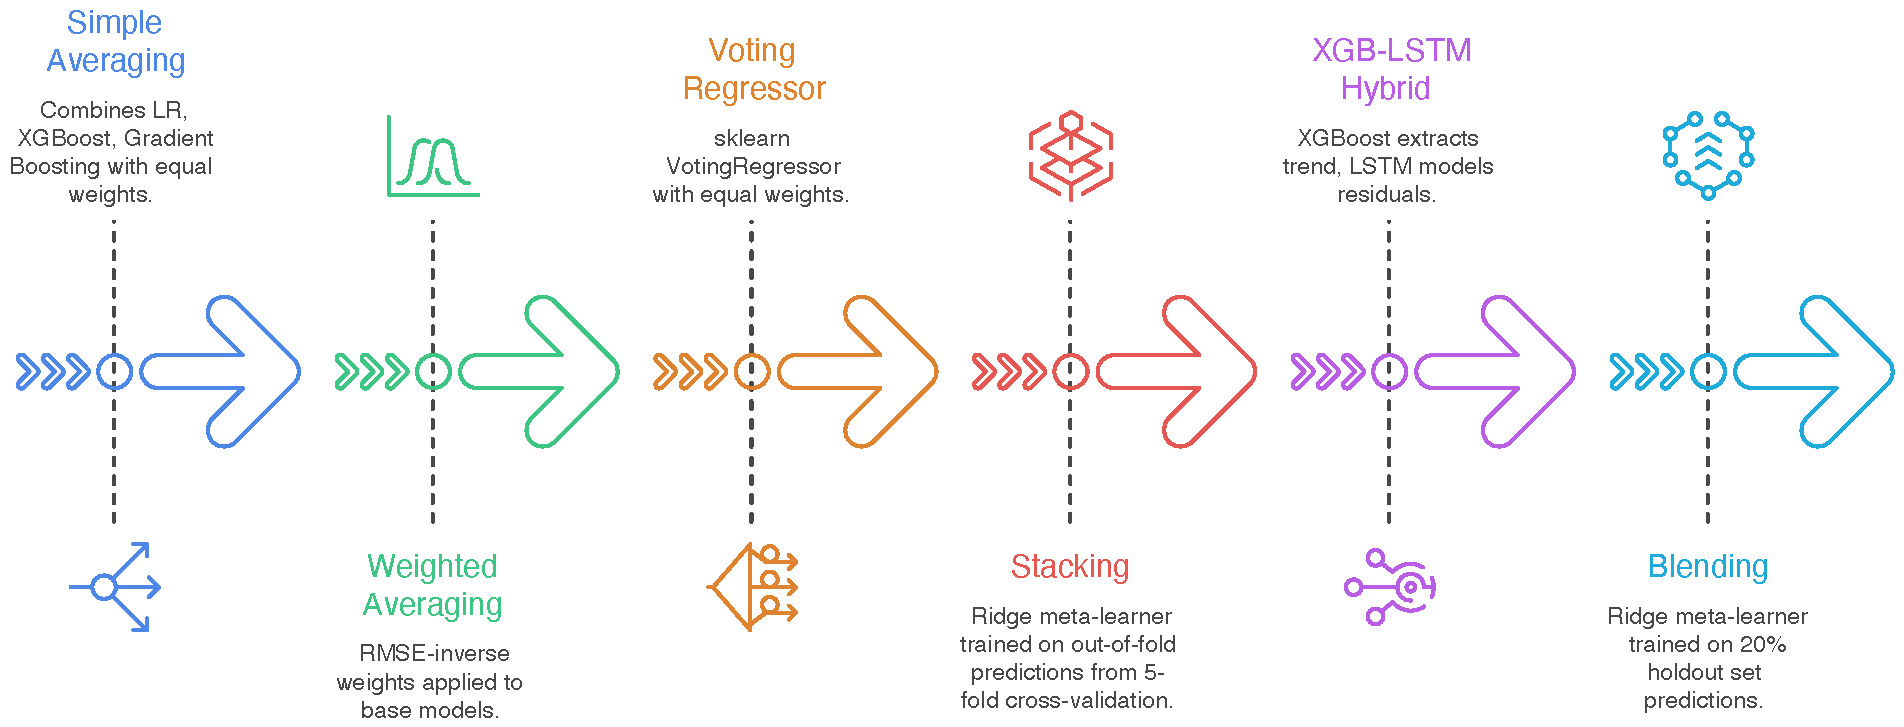
\includegraphics[width=\textwidth, height=0.55\textheight, keepaspectratio]{Figures/ensemble_architecture.pdf}
 \caption{Six ensemble model architectures evaluated in this study: (a) Simple Averaging, (b) Weighted Averaging, (c) Voting Regressor, (d) Stacking with out-of-fold meta-learning, (e) XGBoost-LSTM Hybrid, (f) Blending with a held-out validation partition.}
 \label{fig:ensemble}
\end{figure}

\section{LR-LSTM Hybrid Architecture}
\label{sec:lrlstm}

Motivated by \parencite{kim2020hybrid}, the LR-LSTM Hybrid decomposes demand into a linear component and a non-linear residual, as illustrated in \autoref{fig:hybrid}. The model operates in two stages. In Stage~1, the input feature matrix $\mathbf{X}$ is standardised and a Linear Regression model is fitted to extract the deterministic trend, as shown in \eqref{eq:lr_stage1}:
\begin{equation}
 \hat{\mathbf{y}}^{LR} = \tilde{\mathbf{X}}\boldsymbol{\hat{\beta}}, \qquad
 \mathbf{r} = \mathbf{y} - \hat{\mathbf{y}}^{LR}
 \label{eq:lr_stage1}
\end{equation}
In Stage~2, an LSTM network is trained on the residual series $\mathbf{r}$ from \eqref{eq:lr_stage1} using a lookback window of $L{=}10$ steps and the architecture $\texttt{LSTM}(64)\to\texttt{Dropout}(0.2)\to\texttt{LSTM}(32)\to\texttt{Dropout}(0.2)\to\texttt{Dense}(1)$, optimised with Adam at a learning rate of $10^{-3}$ and early stopping with patience equal to 5~\parencite{tensorflow2015}. The final hybrid prediction is given in \eqref{eq:hybrid_combo}:
\begin{equation}
 \hat{\mathbf{y}}^{\text{hyb}} = \hat{\mathbf{y}}^{LR}_{\text{test}} + \hat{\mathbf{r}}_{\text{test}}
 \label{eq:hybrid_combo}
\end{equation}

\begin{figure}[t]
 \centering
 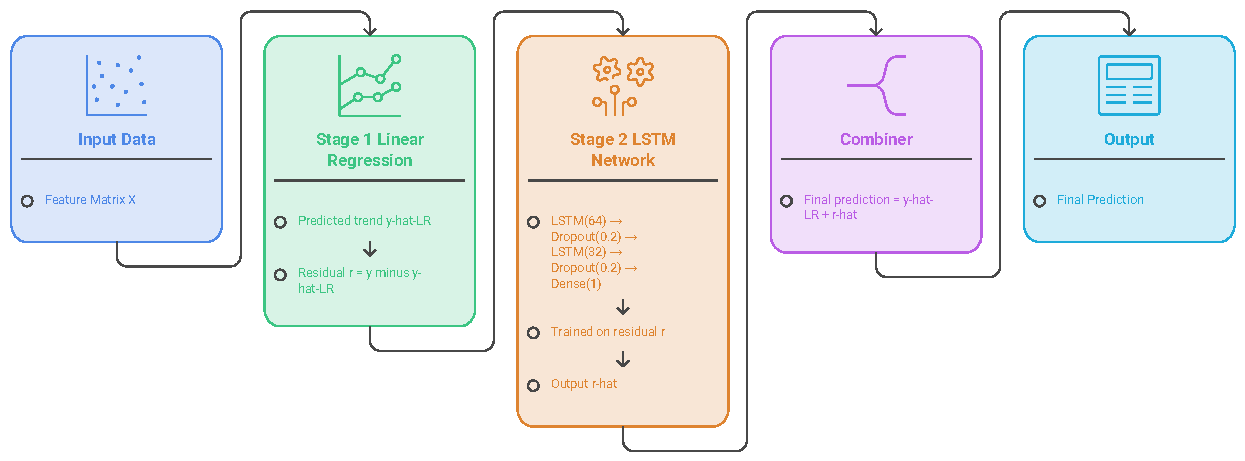
\includegraphics[width=\textwidth, height=0.42\textheight, keepaspectratio]{Figures/hybrid_architecture.pdf}
 \caption{LR-LSTM Hybrid architecture: Stage~1 (Linear Regression) extracts the deterministic trend; Stage~2 (LSTM) models the non-linear residuals.}
 \label{fig:hybrid}
\end{figure}

\section{Ensemble Strategies}
\label{sec:ensembles}

\autoref{fig:ensemble} illustrates the six ensemble strategies evaluated in this study.

The six strategies span a spectrum from parameter-free aggregation to learned meta-combination. Panels~(a)--(c) represent direct aggregation methods: Simple Averaging applies equal weights, Weighted Averaging scales each model's contribution inversely to its validation RMSE, and the Voting Regressor delegates the combination to scikit-learn's built-in implementation. These three methods share the same set of base estimators and differ only in how their predictions are merged; as a result, their test-set performance is closely clustered. Panel~(d), Stacking, is the most sophisticated direct combination strategy: a Ridge meta-learner is trained on out-of-fold predictions produced by 5-fold cross-validation, which ensures that the meta-model never sees in-sample predictions during training and therefore generalises to unseen data. Panel~(e), the XGBoost-LSTM Hybrid, replaces the linear first stage of the LR-LSTM with XGBoost to provide a stronger non-linear trend predictor before residual modelling. Panel~(f), Blending, trains base models on 80\% of the data and uses their predictions on the remaining 20\% holdout to train the meta-learner, providing a simpler but potentially noisier alternative to Stacking. The architectural diversity across these six strategies is deliberate: different inductive biases produce models whose errors are partially independent, and combining partially independent errors is the mechanism through which ensemble methods improve upon any individual constituent.

\paragraph{Simple Averaging.} Equal-weight average of LR, XGBoost, and Gradient Boosting~\parencite{scikit-learn}:
\begin{equation}
 \hat{y}^{SA} = \frac{1}{3}\sum_{k \in \{LR, XGB, GB\}} \hat{y}^{(k)}
 \label{eq:simple_avg}
\end{equation}

\paragraph{Weighted Averaging.} Weights inversely proportional to validation RMSE~\parencite{breiman2001rf}:
\begin{equation}
 w_k = \frac{1/\text{RMSE}_k}{\sum_j 1/\text{RMSE}_j}, \quad \hat{y}^{WA} = \sum_k w_k \hat{y}^{(k)}
 \label{eq:weighted_avg}
\end{equation}

\paragraph{Voting Regressor.} Scikit-learn \texttt{VotingRegressor} with LR, XGBoost, and Gradient Boosting base estimators. Under equal weights this coincides with the Simple Averaging predictor in \eqref{eq:simple_avg}.

\paragraph{Stacking.} Following \parencite{wolpert1992stacking}, base models generate out-of-fold predictions via 5-fold CV; these predictions form a meta-feature matrix $\mathbf{Z}\in\mathbb{R}^{n\times M}$. A Ridge meta-learner solves the regularised objective in \eqref{eq:stacking}, and the stacked forecast follows \eqref{eq:stack_pred}. Algorithm~\ref{alg:stacking} formalises this procedure.
\begin{align}
 \boldsymbol{\hat{\alpha}} &= \arg\min_{\boldsymbol{\alpha}}\,
 \|\mathbf{y}-\mathbf{Z}\boldsymbol{\alpha}\|_2^2 + \lambda\|\boldsymbol{\alpha}\|_2^2,
 \label{eq:stacking} \\
 \hat{\mathbf{y}}^{\text{stack}} &= \mathbf{Z}_{\text{test}}\boldsymbol{\hat{\alpha}}.
 \label{eq:stack_pred}
\end{align}

\begin{algorithm}[H]
\caption{Stacking Ensemble (Meta-Learning via 5-Fold CV)}
\label{alg:stacking}
\begin{algorithmic}[1]
\Require Base models $\{f_1,\ldots,f_M\}$; meta-model Ridge($\alpha{=}1$); data $(\mathbf{X},\mathbf{y})$, test $\mathbf{X}_{\text{test}}$
\Ensure Meta-learned prediction $\hat{\mathbf{y}}^{\text{stack}}$
\State Initialise meta-feature matrix $\mathbf{Z}\in\mathbb{R}^{n\times M}$
\For{each fold $k = 1,\ldots,5$}
 \For{each base model $f_m$}
 \State Train $f_m$ on $\mathbf{X}_{\text{train}\setminus k}$; predict $\mathbf{Z}_{k,m}\gets f_m(\mathbf{X}_k)$
 \EndFor
\EndFor
\State $\boldsymbol{\hat{\alpha}} \gets \arg\min_{\boldsymbol{\alpha}}\,\|\mathbf{y}-\mathbf{Z}\boldsymbol{\alpha}\|_2^2 + \lambda\|\boldsymbol{\alpha}\|_2^2$
\State $\mathbf{Z}_{\text{test}} \gets \bigl[f_m(\mathbf{X}_{\text{test}})\bigr]_{m=1}^{M}$
\State \Return $\hat{\mathbf{y}}^{\text{stack}} \gets \mathbf{Z}_{\text{test}}\boldsymbol{\hat{\alpha}}$
\end{algorithmic}
\end{algorithm}

\paragraph{XGBoost-LSTM Hybrid.} Replaces Stage~1 LR with XGBoost, providing a stronger non-linear first-stage predictor before residual LSTM modelling. The combined forecast is given in \eqref{eq:xgblstm}:
\begin{equation}
 \hat{\mathbf{y}}^{\text{XGB-LSTM}} = \hat{\mathbf{y}}^{\text{XGB}} + \hat{\mathbf{r}}^{\text{LSTM}}.
 \label{eq:xgblstm}
\end{equation}

\paragraph{Blending.} A 20\% holdout partition trains base models on the remaining 80\%; their holdout predictions form a meta-feature matrix $\mathbf{Z}^{\text{hold}}$ used to fit Ridge coefficients $\boldsymbol{\hat{\alpha}}^{\text{hold}}$. The blended test prediction in \eqref{eq:blending} avoids the cross-validation partitioning artefacts of Stacking:
\begin{equation}
 \hat{\mathbf{y}}^{\text{blend}} = \mathbf{Z}^{\text{test}}_{\text{hold}}\,\boldsymbol{\hat{\alpha}}^{\text{hold}}.
 \label{eq:blending}
\end{equation}

\subsection{When Stacking Outperforms Blending, and Vice Versa}

Stacking and Blending represent the two dominant meta-learning paradigms in ensemble literature~\parencite{wolpert1992stacking}, differing in how meta-features are generated. Stacking uses out-of-fold predictions from $K$-fold cross-validation, ensuring that every training observation receives a prediction from a model that was not trained on that observation; Blending uses a single holdout partition, training base models on 80\% and generating meta-features from the remaining 20\%. The trade-off is bias versus variance in the meta-learner training set.

Stacking is preferable when the primary objective is minimising aggregate squared error (RMSE, R\textsuperscript{2}). Out-of-fold meta-features cover the entire training set, giving the Ridge meta-learner more observations to estimate combination weights and reducing the risk that a single holdout partition happens to over-represent a particular demand regime (e.g.\ a holiday week or a snow day). The results in \autoref{tab:results_full} confirm this: Stacking achieves the best RMSE (4.3008), and R\textsuperscript{2} (0.9922). Stacking is also preferable when base models have correlated errors in specific temporal segments: the meta-learner can assign negative or near-zero weights to redundant base models, diversifying predictions beyond what fixed-weight averaging achieves.

Blending is preferable when the primary objective is minimising proportional or log-scale error (MAPE, RMSLE). The holdout partition may better represent the test-set demand distribution if the chronological split places structurally similar periods in the holdout and test sets. Blending's simpler construction also reduces implementation complexity and training time: base models are trained once on 80\% of the data rather than five times across folds. The results confirm that Blending leads on MAPE (9.30\%), and RMSLE (0.1226), likely because the holdout-based meta-training regularises predictions in low-demand cluster-time-bins where proportional deviations dominate the loss function.

For operators, the practical recommendation is metric-aligned selection: deploy Stacking when dispatch decisions depend on absolute pickup counts (e.g.\ ``deploy 15 vehicles to cluster 12 in the next 10 minutes''); deploy Blending when service-level agreements are expressed as percentage accuracy (e.g.\ ``forecast within 10\% of actual demand''). When computational budget is constrained and cross-validation overhead is prohibitive, Blending offers a simpler alternative with competitive performance on percentage metrics. When maximum accuracy is required and training time is not a bottleneck, Stacking is the stronger choice on aggregate error.

Simple and weighted averaging remain valuable as interpretable baselines: they require no meta-learner training, produce transparent combination weights, and achieve RMSE within 10\% of Stacking in the present experiments. For deployment contexts where model interpretability and auditability are required, such as regulatory reporting or stakeholder communication, a weighted average of three well-understood base models may be preferable to a black-box stacking meta-learner, despite the modest accuracy sacrifice.

\section{Design Rationale and Alternatives}
\label{sec:framework-rationale}

The EnsembleNet framework adopts a modular two-tier architecture, individual models followed by ensemble meta-learning, rather than pursuing a single end-to-end deep architecture. This design choice reflects three considerations grounded in the experimental evidence and the literature reviewed in \autoref{ch:related}.

First, tabular spatio-temporal features with engineered lags and cyclical encodings are well suited to gradient-boosted trees~\parencite{chen2016xgboost}, which achieve the strongest individual performance in this study. End-to-end deep models such as ST-ResNet~\parencite{zhang2017deep} or graph convolutions~\parencite{li2018diffusion} require converting the cluster-bin representation into grid or graph structures, introducing preprocessing complexity and data requirements (road topology) absent from the NYC trip records. The modular pipeline preserves direct comparability with the Kim et al.~\parencite{kim2020hybrid} benchmark and avoids architectural commitments that would prevent fair cross-model comparison.

Second, ensemble meta-learning is empirically superior to any single model or hybrid variant in the present experiments. Stacking and Blending both outperform the LR-LSTM and XGBoost-LSTM hybrids on RMSE, confirming that combining diverse model families captures complementary error structure that residual decomposition alone cannot address. The six ensemble strategies span a spectrum from parameter-free (Simple Averaging) to learned (Stacking, Blending), enabling practitioners to select complexity appropriate to their deployment context.

Third, the Ridge meta-learner with $\alpha{=}1.0$ is chosen over more flexible meta-models (e.g.\ XGBoost or neural networks) to prevent meta-level overfitting. With only seven base models generating meta-features, a regularised linear meta-learner is unlikely to overfit the meta-feature space, whereas a non-linear meta-learner with limited meta-training observations could memorise fold-specific artefacts. This conservative choice aligns with stacking best practices~\parencite{wolpert1992stacking} and is validated by the tight cross-validation RMSE distributions reported in \autoref{tab:kfold}.

Alternatives considered but not adopted include: (i)~a single end-to-end LSTM without linear pre-processing, rejected because~\parencite{xu2017realtime} showed LSTM superiority over feed-forward models but the present linear-first hybrid achieves comparable MAPE with better interpretability; (ii)~a deep ensemble of neural networks, rejected due to training time and the strong tabular performance of gradient-boosted trees; (iii)~a dynamic ensemble that selects models by time-of-day regime, rejected because Stacking's Ridge meta-learner already learns regime-dependent weights implicitly through the meta-feature coefficients. The modular architecture ensures that each of these alternatives can be substituted in future work without redesigning the pooling or evaluation components of the pipeline.
